\chapter{Which Python version?}

You should be porting from Python 2.7, there is no doubt about this. After all, 2.6 support has ended in 2013.

However, I had a client in 2018 that was still using a code base with idioms dating from Python 2.5, so there may be some of you that have a few pieces of very old Python out there, espacially if you use very old Unix systems.

There is no use to try to migrate from an earlier version directly to Python 3. So if you are unlucky enough to have inherited a very deprecated legacy code base, your first mission will be to migrate to 2.7. This version being forward compatible with older ones, you should be fine: the bulk of the work will probably be your dependances and clearing a few odities such as in classes and try/excepts.

Before you start, you need to decide which Python 3 version you are going to target. Since you are migrating to an imcompatible version anyway, I advice to choose the highest version your technical constraints allow you to.

\section{Overview of the releases}

\subsection{Python 3.0 to 3.2}

Do not use those versions. They are very limited and badly supported.

\subsection{Python 3.3, 3.4}

The first Python 3 releases you could reasonably put in production. You will also find them in old Unix distributions official repositories. The 3.4 is the last one to support Windows XP, if that's important to you.

Most importantly, the 3.4 is the first release to come bundled with a pip installer\footnote{Either directly in the Python installer, or through the ensurepip module} on non Linux systems\footnote{A lot of Linux distributions, such as Debian and Fedora based ones, have a separate package for pip you still must install manually today}.

While Python 3.4 introduces the excellent \href{https://docs.python.org/3/library/pathlib.html}{pathlib} and \href{https://docs.python.org/3/library/asyncio.html}{asyncio} libraries, they are not well integrated and full of gotchas. If you plan to use those libraries, use higher Python versions.

3.4 is slowly being abandonned at the same time as 2.7. NumPy 1.16 and Django 2.1 both have dropped Python 3.4 support.

Use those versions if you have no other choices.

\subsection{Python 3.5}

This is the earlier version you want if you work with the network a lot.

It's the first version to restore formatting with the \lstinline{\%} operator for bytes, and also to introduce the \lstinline{await}/\lstinline{async} keywords, making \lstinline{asyncio} much more usable. However, if you want to use the module, make sure you can guaranty at least Python 3.5.3 as not only it sets \lstinline{TCP_NODELAY} by default\footnote{Which result to up to X30 of performance gain with network calls}, but an important bug has been fixed on \lstinline{get_event_loop()}\footnote{Before this, \lstinline{get_event_loop()} didn't always return the proper loop when threads where involved}.

\subsection{Python 3.6}

This version is what motivated a lot of people to start their own migration, as it's very feature rich and handy. If you can target this one, you'll get:

\begin{itemize}
\item A well integrated \lstinline{pathlib}, making any file system operation a breath.
\item Dictionaries preserving insertion order. Yes it's not official, but it won't change, so you can use it as if it were.
\item UTF8 by default on Windows.\footnote{Before that, opening a file on Windows had a different behavior than on other OS, resulting in a lot of confusion}
\item A well behaved \lstinline{asyncio}.
\item f-string, which makes text formatting incredibly nice.
\end{itemize}

And generally many little fixes that make it so comfortable, but honestly f-string are worth it by themselves !

Because it's such a good release, some great projects such as \href{https://github.com/psf/black}{black}\footnote{black automatically format your code and is becomming very popular has it's been adopted by many major Python open source projects. If you are not using it now, check it out.} only support python 3.6+. It's another good reason to target it.

It can be easier to install than you expect, as it came out in late 2016, giving time for support, so definitly give it a try.

\subsection{Python 3.7 and 3.8}

The most moderne releases at the time of writting, introducing goodies such as a Python debug mode, a shorter syntax for classes, more performances and a quicker \lstinline{asyncio} setup code.

Your project probably doesn't need those, but they are nice to have.

\section{Installation methods for your new version of Python}

Since choosing which version to target is related to the plateform you will dev or deploy on, let's see what are your options to install a modern Python on your machines.

If you are on Windows or Mac, the official installer are the best way to go. Alternatively, Windows 10 app store and Mac OS's \href{https://brew.sh/index_fr}{homerewb} both allow you to install Python 3.7.

In fact, if you type \lstinline{python} in a Windows terminal and no Python is installed, it will take you to the app store to install it.

If one of this two is your OS, then you should be able to choose the most recent Python version to date. Unless you have other very specific constraints, please do.

The only thing to check is that you install the 64 bits version of Python: migrating to a modern Python and yet keeping a 32 bits build is probably not what you want. Be warned: the most featured download link on \href{https://python.org}{python.org} may be a 32bits installer. Double check, and if needed, browse manually \href{https://www.python.org/downloads/}{the download section of the site}.

\begin{warning}
    Mac and Linux distributions come with a bundled Python, but it will most probably be Python 2.7.
\end{warning}

If you use your linux distribution official repositories, chances are that you won't be able to install the most modern version of Python. If it's alright with you, good.

However, remember you always have the option to use the \href{https://fedoraproject.org/wiki/EPEL}{EPEL repositories} for Fedora based distros (\footnote{I managed to install Python 3.6 on Cent OS 7 without much effort} and the \href{https://launchpad.net/~deadsnakes/+archive/ubuntu/ppa}{deadsnake PPA} for Ubuntu based ones \footnote{Starting from the 16.04 it provides Python 3.7}.

If none of that works for you, the \href{https://github.com/pyenv/pyenv}{pyenv} project will let you install an arbitrary Python version by compling it for you automatically. It's a bit work to setup, but it's not very hard, and may give you access to recent Python versions on unexpeted plateforms.

So even on GNU/Linux, you have options to still use a recent version of Python. Aim for that.

\begin{warning}
    Trying to compile Python yourself is not something I would recommand, unless you really know what you are doing. It's surprisingly easy to do, but also easy to get wrong. Python has many configuration knobs and optional dependancies you are likely not going to setup properly. What's more, the default behavior is to replace your system Python, which will cause all sorts of troubles. I learned the hard way that \lstinline{yum} is coded in Python, and that once I replaced my system Python with a badly compiled one, there is not much I could do to fix my server. If you still want to do it, check that you know all optional dependancies (libcurse, readline, gdb, libdb, sqlite, ssl, zlib, lzma, etc) and that on Unix, you do \lstinline{make altinstall} and not \lstinline{make install}.
\end{warning}

\section{Having several Python versions side by side}
--------------------------------------------

Since you are moving from one version to another, you will have several of them installed on your computer. Python has been designed for that use case, and barring a very messed up configuration, there is nothing to do on your part for it to work: you can just install python 2 and Python 3 as usual.

However, calling the proper Python is another matter.

If you are on Mac or Linux, the \lstinline{python} command is generally 2.7 by default. But luckily you also have aliases with a suffix containing a version number, so you can just call \lstinline{python2.7} or \lstinline{python3.6} to use the exact version you want.

If you are on Windows, there is a little tick box in the official installer asking you if you want to add Python to the system PATH:

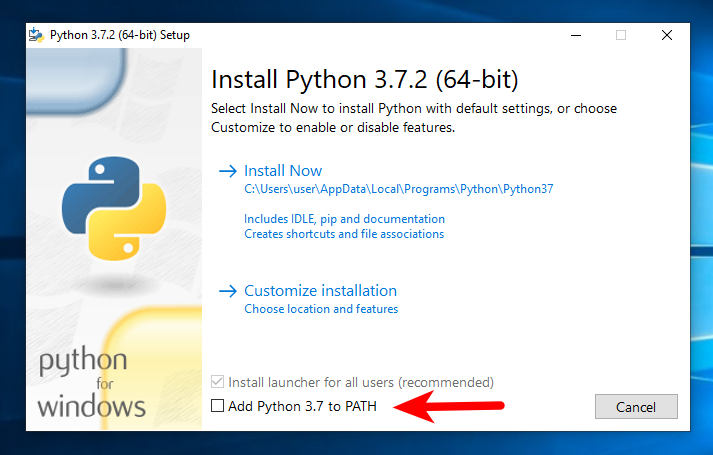
\includegraphics[width=\textwidth,height=\textheight,keepaspectratio]{python37_win_installer.png}

This box is not ticked by default, but if you don't tick it, you won't be able to type the \lstinline{python} command in a terminal, so either people tick it, add the Python installation directory manually to the system PATH, or type the full path to the Python executable.\footnote{if you choose Anaconda as a distribution, they provide a \textquote{Python console} entry in the Windows \textquote{Start} menu and their launcher to bypass this exact problem}

Adding \lstinline{python} to the system PATH works fine if you have only one Python version installed, but Windows Python executable don't have a version suffix, so if you install several Python, only one can get called from the command line: the last one added to the PATH.

To work around this, modern Python installers provide another tool on Windows, the \lstinline{py} command, which can be used just like the \lstinline{python} command (down to the same options and arguments), except you can pass a version to it: \lstinline{py -2.7} will start Python 3.7, while \lstinline{py -3.5} will start Python 3.5.

\begin{warning}
To simplify things, I will always use the \lstinline{python} command in this book. Replace it mentally with what's appropriate for you, wether it's \lstinline{python3.7} for Linux/Mac/etc or \lstinline{py -3.7} for Windows. All options and syntaxes remain the same.
\end{warning}

\section{Using a virtual environement}

As stated in the intro, the book will not explain how to use pip and virtualenv and expect you to know how.

But since you will use several Python versions, I strongly advise you to setup at least two virtual environements, one for Python 2.7, and once for Python 3.X, X depending of the version you want to port to.

I would setup two separated versions of the code, preferably using a two clones from your Version Control System (Git, Mercurial, SVN, etc) on different branches. If you don't use a VCS, now maybe a good time to learn, before starting the migration.

If you really won't use a VCS, just copy the entire code in a separate directory.

Having those 2 separate silos of code  will make things easier than having to go back and forth from one version to the other: your port may stay broken for a while during the migration, and you will probably need to fix things on the working one during that time.
